\documentclass[11pt,letterpaper]{article}
%\usepackage[T1]{fontenc}
%\usepackage[utf8]{inputenc}
\usepackage[margin=1in]{geometry}
\usepackage{ragged2e,booktabs,multirow}
\usepackage{caption,capt-of}
\usepackage{graphicx}
\usepackage{array}
\renewcommand{\thetable}{S\arabic{table}}
\renewcommand{\thefigure}{S\arabic{figure}}

\newcolumntype{M}[1]{>{\begin{varwidth}[t]{#1}}l<{\end{varwidth}}}

\RequirePackage[LY1]{fontenc}

\renewcommand{\rmdefault}{ptm}
\renewcommand{\sfdefault}{phb}
\renewcommand{\ttdefault}{pcr}

%\RequirePackage[LY1,mtbold]{mathtime}
\def\helvetica{\fontfamily{phv}\selectfont}
\def\helveticaitalic{\fontfamily{phv}\itshape\selectfont}
\def\helveticabold{\fontfamily{phv}\bfseries\selectfont}
\def\helveticabolditalic{\fontfamily{phv}\bfseries\itshape\selectfont}
\def\helveticacn{\fontfamily{phv}\fontseries{mc}\fontshape{n}\selectfont}
\def\helveticacnitalic{\fontfamily{phv}\fontseries{mc}\fontshape{sl}\selectfont}
\def\helveticacnbold{\fontfamily{phv}\fontseries{bc}\fontshape{n}\selectfont}
\def\helveticacnbolditalic{\fontfamily{phv}\fontseries{bc}\fontshape{sl}\selectfont}

\title{Phylotyper: {\it In silico} predictor of molecular subtypes from gene sequences \\ \large Supplementary Information}
\author{Matthew D. Whiteside, Chad R. Laing and Victor P.J. Gannon}
\date{ }


\begin{document}
 
%\maketitle
 
\tableofcontents

\clearpage

\section{Supplementary Methods}

\subsection{Performance Analysis}

\subsubsection{BLAST-based method}

BLAST 

\subsubsection{Selecting Percent Identity Cutoff for BLAST Approach}

Following \citep{Jenkins2015}, percent identity in the BLAST alignments is used as a cutoff. Subtype classifications are transfered from the top BLAST match provided the alignment percent identity is above the cutoff. The cutoff impacts performance in one of two ways: too low and non-equivalent subtype alleles may be matched with the query (e.g. type I error), too high and valid subtype allele BLAST hits are filtered out (e.g. type II error). To select the ideal cutoff that balances these competing sources of error, a cross-validation simulation was run to estimate false discovery and true positive rates across varying percent identity cutoffs. A 10-fold cross-validation was performed; 10\% of the training set was randomly selected. The remaining 90\% was used to build the reference BLAST database. The 10\% test set was then searched against this database using BLAST and positive and negative results were recorded. This step was repeated 100 times and the F1-score, which is a weighted average of the precision and recall, was calculated. Precision is defined as: 

$Precision = TP / (TP + FP)$

and recall as:

$Recall = TP / (TP + FN)$

These values are then combined to produce an F-score as follows:

$2 * ( precision * recall ) / ( precision + recall )$

The F-score; a binary classifer metric, was recorded individually for each subtype and then averaged to create a single performance metric for this multi-class predictor.  F-score was computed for increasing percent identities, and the percent identity corresponding to the maximum F-score was selected as the cutoff.

\subsubsection{Performance Assessment}

Two separate cross-validation tests were performed to compare the performance of Phylotyper with the BLAST method. The comparison to vtyper is a separate analysis, as vtyper does not use a training set and a cross-validation test would not work in this situation. A leave-one-out cross-validation analysis was performed where each sequence in the training set is withheld and the remaining sequences are used for form the phylogenetic tree for Phylotyper or are used to build the BLAST database for the BLAST-based approach. The predicted result for the test sequence is then compared to the true value.

\subsubsection{V-typer Assessment}

The V-typer tool predicts Stx1 or Stx2 subtypes by simulating PCR (i.e. mapping primers). Due to the unique method in V-typer,  which does not use a training dataset, the cross-validation assessment was adapted to test V-typer. Each experimentally-verified Stx gene sequence that makes up Phylotyper training dataset was searched for against the NCBI nt database to retrieve surrounding sequence that may be involved in the PCR detection by V-typer.  Specifically, regions that have at least 5 kB up- and downstream from the Stx gene were selected for the assessment. V-typer was run on each sequence and the results recorded in supplmentary table XXXX.


\section{Supplementary Figures}

\subsection{Supplementary Figure S1}

\begin{figure}[h!]
\centering
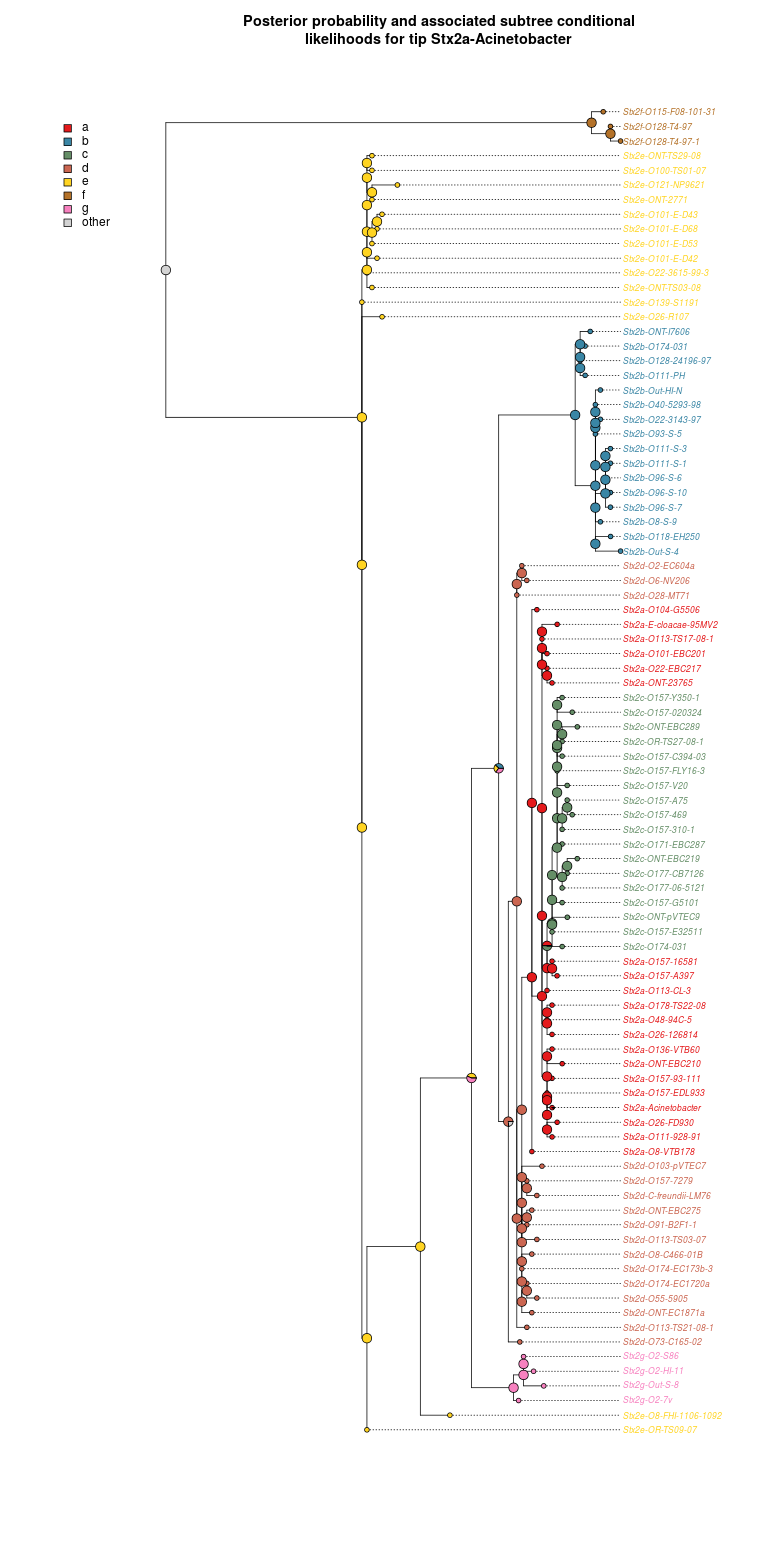
\includegraphics[scale=0.5]{sfig01.png}
\caption{Stx2 Phylogenetic tree showing the Phylotyper marginal likelihoods as pie charts. This output is provided to the user.}
\end{figure}

\clearpage

\section{Supplementary Tables}

\subsection{Supplementary Table S1}

~

\begin{minipage}{\linewidth}
\centering
\captionof{table}{Subtype Schemes in Phylotyper}
\medskip
\begin{tabular}{@{}llll@{}}\toprule Name &
Description & Species & Loci\\\midrule
stx1 & Shiga-toxin 1 subtype & {\it E. coli} & 2 \\
stx2 & Shiga-toxin 1 subtype & {\it E. coli} & 2\\
eae & Intimin subtype & {\it E. coli} & 1\\
flic & H-serotype based on flagellin gene; fliC & {\it E. coli} & 1\\
wz & O-serotype based on the wzy and wzx genes & {\it E. coli} & 2\\\bottomrule
\end{tabular}\par

\end{minipage}

\clearpage

\subsection{Supplementary Table S2}

Table S2 contains performance metrics from a leave-one-out cross-validation analysis comparing Phylotyper and a top-BLAST hit approach.  The analysis examines the four \textit{E. coli} schemes available in Phylotyper. In this multi-class analysis, precision, recall and F$_{1}$ score are calculated for each individual class provided that at least one instance of the class is in the training set.  The individual class positive and negatives are summed to calculate an overall precision, recall and F$_{1}$ score for the scheme.

%\captionsetup{justification=RaggedRight}

\begin{minipage}{\linewidth}
\centering
\setlength{\tabcolsep}{4pt}
\captionof{table}[justification=RaggedRight]{Leave-One-Out Cross Validation Results}
\medskip
\begin{tabular}{@{\extracolsep{4pt}}llll>{\centering}m{1.6cm}lll@{}}
\toprule 
\multirow{2}{*}{Scheme} & \multicolumn{4}{c}{Phylotyper} & \multicolumn{3}{c}{Sequence-similarity}\\
\cline{2-5}\cline{6-8}
& Precision & Recall & F$_{1}$ Score & Run-time (s) $^{1}$ & Precision & Recall & F$_{1}$ Score \\
\midrule
{\it E. coli} Stx1 & 1.00 & 0.94 & 0.97 & 6 & 0.94 & 0.94 & 0.94\\
{\it E. coli} Stx2 & 1.00 & 0.99 & 0.99 & 32 & 0.93 & 0.93 & 0.93\\
{\it E. coli} Intimin & 1.00 & 0.98 & 0.99 & 17 & 0.99 & 0.98 & 0.99\\
{\it E. coli} H-serotype & 0.99 & 0.98 & 0.98 & 16 & 0.96 & 0.85 & 0.90\\
{\it E. coli} O-serotype & 1.00 & 0.61 & 0.75 & 67 & 1.00 & 0.36 & 0.53\\\bottomrule
\end{tabular}\par
\bigskip
\raggedright
Formula:
\begin{enumerate}
\item $Precision = TP / (TP + FP)$
\item $Recall = TP / (TP + FN)$
\item $F_{1}~score = 2*Precision*Recall/(Precision + Recall)$
\end{enumerate}
$TP = True~Positive,~~FP = False~Positive,~~FN = False~Negative$
\par
\bigskip
$^{1}$ Run-time is for an {\it Escherichia coli} genome containing a unique gene which triggers the full phylotyper pipeline.

\end{minipage}

\begin{minipage}{\linewidth}
\centering
\captionof{table}{V-typer Performance}
\medskip
\begin{tabular}{@{}llll@{}}\toprule
NCBI Accession & Stx Subtype & V-typer Prediciton$^{1}$ & Phylotyper Prediction\\\midrule
CP015020 & 2d & N & 2d \\
CP015229 & 2g & 2g & 2g \\
CP009106 & 2a & N & 2a \\
CP007133 & 2a & 2a & 2a \\
CP006262 & 2a & 2a & 2a \\
AP010960 & 2a & 2a & 2a \\
CP013663 & 2a & N & 2a \\
CP015228 & 2a & N & 2a \\
CP011331 & 2a & N & 2a \\
HF572917 & 2a & N & 2a \\
LN554923 & 2a & N & 2a \\
LM997071 & 2a & N & 2a \\
CP018250 & 2c & N & 2c \\
CP018252 & 2c & N & 2c \\
CP018247 & 2c & N & 2c \\
CP018245 & 2c & N & 2c \\
CP018243 & 2c & N & 2c \\
CP017446 & 2c & N & 2c \\
CP017442 & 2c & N & 2c \\
CP017438 & 2c & N & 2c \\
CP014314 & 2c & N & 2c \\
LM997036 & 2a & 2a & 2a \\
LM996489 & 1c & 1c & 1c \\
LM997036 & 1c & 1c & 1c \\
Total & 24 & 7 & 24 \\
\bottomrule
\end{tabular}\par
\bigskip
\raggedright
$^{1}$ N=Negative (no results returned)

\end{minipage}

\end{document}
